
\documentclass[xcolor=pdftex,dvipsnames,table,mathserif,aspectratio=169]{beamer}
\usetheme{default}
\usetheme{metropolis}
\usepackage{ulem}
%\usepackage{minted}
\usepackage{mathtools}
\usepackage{tikz}
\usepackage{booktabs}
% Tikz settings optimized for causal graphs.
% Just copy-paste this part

\setbeamersize{text margin left=.3in,text margin right=.3in} 

\DeclarePairedDelimiter\abs{\lvert}{\rvert}%
\DeclarePairedDelimiter\norm{\lVert}{\rVert}%


%\usetheme{Darmstadt}
%\usepackage{times}
%\usefonttheme{structurebold}

\usepackage[english]{babel}
%\usepackage[table]{xcolor}
\usepackage{pgf,pgfarrows,pgfnodes,pgfautomata,pgfheaps}
\usepackage{amsmath,amssymb,setspace,centernot}
\usepackage[latin1]{inputenc}
\usepackage[T1]{fontenc}
\usepackage{relsize}
\usepackage{pdfpages}
\usepackage[absolute,overlay]{textpos} 

% math functionality
\usepackage{amsthm}
\usepackage{amssymb}
\usepackage{amsmath}
\usepackage{amsfonts}
\usepackage{amsmath, amsthm, amssymb, amsfonts}
\newcommand\leftmapsto{\mathrel{\reflectbox{\ensuremath{\mapsto}}}}

% number equations within at the beginning so cleveref works
%\numberwithin{equation}{section}
\renewcommand{\theequation}{\arabic{equation}}




\newenvironment{reference}[2]{% 
  \begin{textblock*}{\textwidth}(#1,#2) 
      \footnotesize\it\bgroup\color{red!50!black}}{\egroup\end{textblock*}} 

\DeclareMathSizes{10}{10}{6}{6} 

\begin{document}
\title{Part 9: Local Average Treatment Effects Application:\\
 Demand Curves}
\author{Chris Conlon}
\institute{Applied Econometrics}
\date{\today}

\frame{\titlepage}




\begin{frame}{A Classic Example}
\begin{itemize}
\item What is the effect of prices on quantity demanded?
\item But a regression of $\log(q_t)  = \beta_0 + \beta_1 \log(p_t) + u_t$ is going to be flawed.
\item For one thing, how do we know that relationship represents supply or demand?
\item Imagine an instrument $z_t \in \{0,1\}$ that reduces supply but does not effect demand.
\item What about?
\begin{itemize}
\item Monotonicity?
\item Heterogeneity in treatemnt effects?
\item Exclusion Restriction?
\end{itemize}
\end{itemize}
\end{frame}


\begin{frame}
\frametitle{LATE at the Fulton Fish Market (Graddy 1995)}
\begin{center}
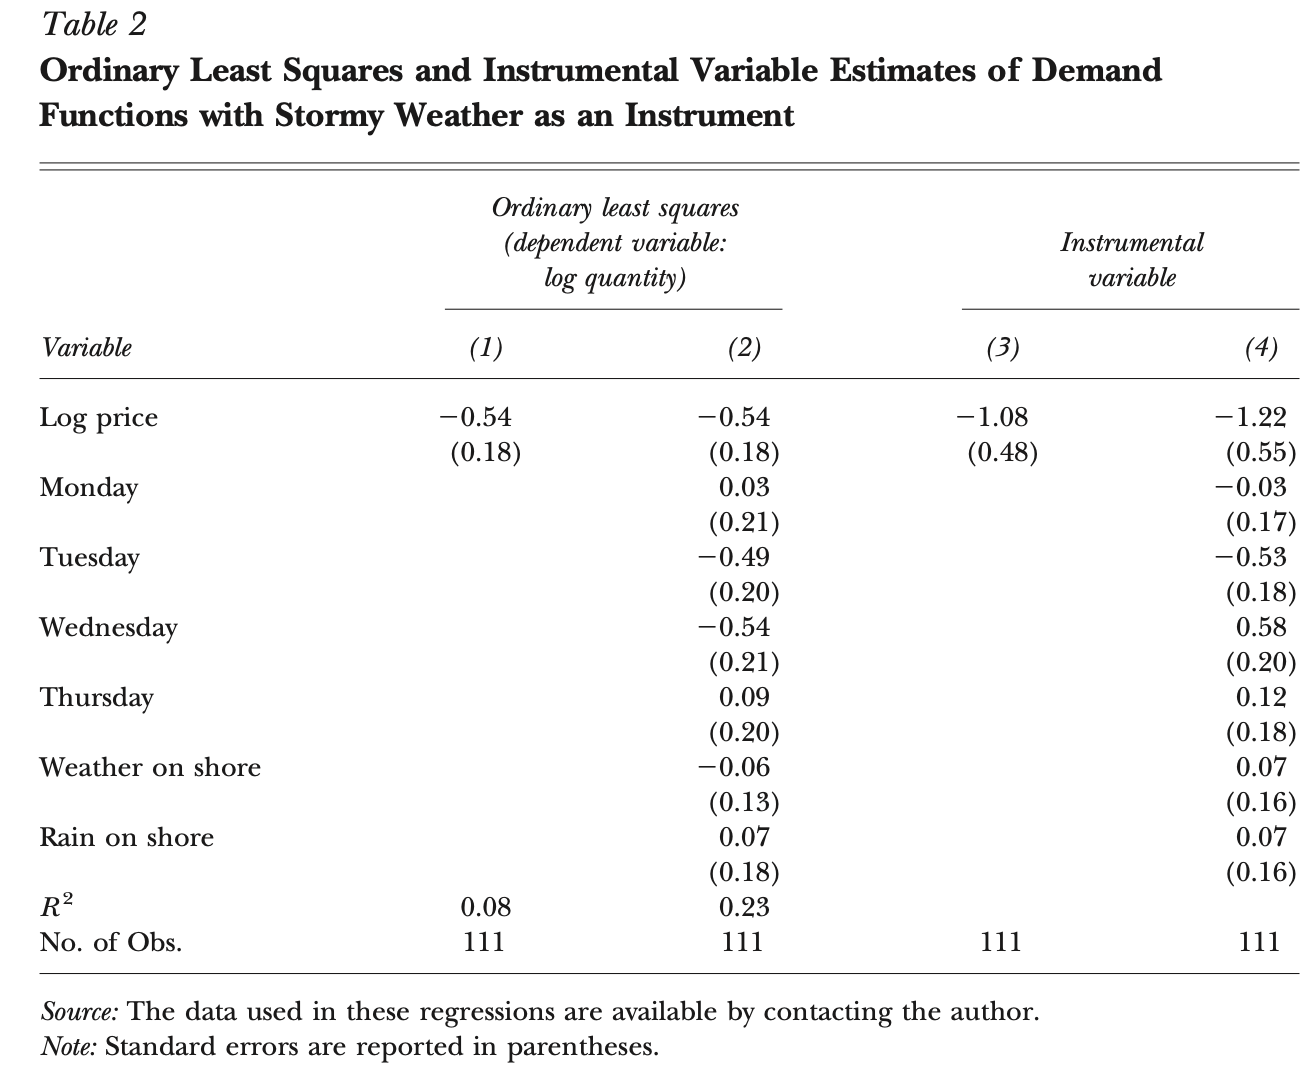
\includegraphics[width=\textheight]{./resources/graddy}
\end{center}
\end{frame}


\begin{frame}{Wald Estimator}
\small
Focus on the simple case:
\begin{itemize}
\item $z_t \in \{0,1\}$ where $1$ denotes ``stormy at sea'' and 0 denotes ``calm at sea''
\item Idea is that offshore weather makes fishing more difficult but doesn't change onshore demand.
\item Ignore $x$ (for now at least) or assume we condition on each value of $x$.
\end{itemize}
\begin{align*}
\hat{\alpha}_{1,0}  \rightarrow^p \frac{\mathbb{E}[q_t | z_t=1] - \mathbb{E}[q_t | z_t=0]}{\mathbb{E}[p_t | z_t=1] - \mathbb{E}[p_t | z_t =0]} \equiv \alpha_{1,0}
\end{align*}
\begin{itemize}
\item If we have homogenous $\alpha$ then any IV gives us a consistent estimate of $\alpha_1$
\item If we are in complicated (nonlinear, heterogeneous) then $\alpha_{1,0}$ the object we recover, is not an estimator of a structural parameter.
\item Moreover, this is at best a LATE, and thus it differs depending on which instrument we use!
\end{itemize}
\end{frame}


\begin{frame}{AIG: Assumptions}
\begin{enumerate}
\item Regularity conditions on $q_t^d, q_t^s,p_t,z_t,w_t$ first and second moment and is stationary, etc.
\begin{itemize}
\item  $q_t^d(p,z,x)$ ,  $q_t^s(p,z,x)$ are continuously differentiable in $p$.
\end{itemize}
\item $z_t \in \{0,1\}$ is a valid instrument in $q_t^d$
\begin{itemize}
\item Exclusion: for all $p,t$ 
\begin{eqnarray*}
q_t^d(p,z=1,x_t) = q_t^d(p,z=0,x_t) \equiv q_t^d(p,x_t)
\end{eqnarray*}
ie: conditioning on $p_t$ means no dependence on $z_t$
\item Relevance: for some period $t$: $q_t^s(p_t,1,x_t) \neq q_t^s(p_t,0,x_t)$.\\
ie: $z_t$ actually shifts supply somewhere!
\item Independence: $\epsilon_t, \eta_t, z_t$ are mutually independent conditional on $x_t$.
\end{itemize}
\end{enumerate}
\end{frame}


\begin{frame}{AGI: Structural Interpretation}
In order to interpret the Wald estimator $\alpha_{1,0}$ we make some additional \alert{economic} assumptions on the structure of the problem:
\begin{enumerate}
\item Observed price is market clearing price $q_t^d(p_t) = q_t^s(p_t,z_t)$ for all $t$. (This means no frictions!).
\item ``Potential prices'': for each value of $z$ there is a unique market clearing price
\begin{eqnarray*}
\forall z,t : \tilde{p}(z,t) \mbox{ s.t. } q_t^d(\tilde{p}(z,t)) = q_t^s(\tilde{p}(z,t),z).
\end{eqnarray*}
\end{enumerate}
$\tilde{p}(z,t)$ is the potential price under any counterfactual $(z,t)$
\end{frame}


\begin{frame}{AGI: Structural Interpretation}
\begin{itemize}
\item Just like in IV we need denominator to be nonzero so that
$E[p_t | z_t=1] \neq E[p_t | z_t = 0]$.
\item Other key assumption is the familiar \alert{monotonicity} assumption
\begin{itemize}
\item $\tilde{p}(z,t)$ is weakly increasing in $z$.
\item Just like in program evaluation this is the key assumption. There it rules out ``defiers'' here it allows us to interpret the \alert{average slope} as $\alpha_{1,0}$.
\item Assumption is untestable because you do not observe both potential outcomes $\tilde{p}(0,t)$ and $\tilde{p}(1,t)$ (same as in program evaluation).
\item Any story about IV is just a story! (Always the case!) unless we have repeated observations on the same individual.
\end{itemize}
\item Monotonicity makes extending to multiple product case difficult/impossible.
\end{itemize}
\end{frame}


\section{Conlon Mortimer RJE (2021)}

\begin{frame}{Wald Estimator: Redux}
Consider the following Wald estimator:
\begin{align*}
\text{Wald}\left(p_{j}, p_{j}^{\prime}, x\right)&=\frac{q_{k}\left(p_{j}^{\prime}, x\right)-q_{k}\left(p_{j}, x\right)}{-\left(q_{j}\left(p_{j}^{\prime}, x\right)-q_{j}\left(p_{j}, x\right)\right)} \\
\lim _{p_{j}^{\prime}  \rightarrow p_{j}} \text{Wald}\left(p_{j}, p_{j}^{\prime}, x\right) &\rightarrow \frac{\frac{\partial q_{k}}{\partial P_{j}}\left(p_{j}, x\right)}{-\frac{\partial q_{j}}{\partial P_{j}}\left(p_{j}, x\right)} \equiv D_{j k}\left(p_{j}, x\right)
\end{align*}
We call $D_{j k}\left(p_{j}, x\right)$ the \alert{Diversion Ratio}.\\
 As we increase $P_j$ and people leave what fraction switch to $k$?
\end{frame}

\begin{frame}{Wald Estimator: Relation to IV Case}
To solidify the connection with the quasi-experimental LATE framework, recognize that our hypothetical price change experiment can be interpreted using the following definitions:
\begin{description}
\item[Outcome] $Y_i \in \{0,1\}$ denotes the event that consumer $i$ purchases product $k$: $d_{ik}(P_j)=1$.
\item[Treatment] $T_i \in \{0,1\}$ denotes the event that consumer $i$ does \textbf{not} purchase product $j$. In other words $T_i = 0$ implies $d_{ij}(P_j)=1$ and $T_i=1$ implies $d_{ij}(P_j)=0$.
\item[Instrument] $Z_i = P_j$ the price of $j$ induces consumers into not purchasing $j$.
\end{description}
\end{frame}


\begin{frame}{Diversion: Why do we care?}
\begin{itemize}
\item Related to \alert{cross price elasticity} $D_{jk} =\frac{\frac{\partial q_{k}}{\partial P_{j}}\left(p_{j}, x\right)}{-\frac{\partial q_{j}}{\partial P_{j}}\left(p_{j}, x\right)} = -\frac{\epsilon_{jk}}{\epsilon_{jj}} \times \frac{q_k}{q_j} $
\item Related to multi-product differentiated Bertrand FOC $(MR = MC)$:
\begin{align*}
p_j(\mathbf{p})\left[1 +  \frac{1}{\epsilon_{jj}(\mathbf{p})}  \right] =  mc_j + \sum_k (p_k -mc_k) \cdot D_{jk} 
\end{align*}
\item $D_{jk} \in [0,1]$ and $\sum_k D_{jk} =1$ and high-diversion ratios indicate close substitutes.
\end{itemize}
\end{frame}

\begin{frame}{Diversion: Assumptions}
Like in multiple discrete choice lectures assume that:
\begin{enumerate}
\item Consumers make mutually exclusive and exhaustive \alert{discrete choice}.
\item Can be guaranteed by presence of an \alert{outside option}.
\item Utility $u_{ij}(x)$ can be \alert{deterministic} or \alert{stochastic}.
\item $x$ contains all covariates that don't change (other prices and characteristics).
\item Could be mixed logit but doesn't need to be...
\begin{align*}
d_{ij}(p_j,x) =\begin{cases} 
1 & u_{ij}(p_j,x) > u_{ij'}(p_j,x) \text{ for all }  j' \in \mathcal{J} \text{ and } j'\neq j.\\
0 & o.w.
 \end{cases}
 \end{align*}
\item $s_{ij }(x) = \int d_{ij}(x) d \, F_i$ (share of individuals choosing $j$) and $q_j(x)= s_j(x) \cdot M$.
\end{enumerate}
\end{frame}

\begin{frame}{Diversion as LATE}
\begin{block}{Analogue to LATE Theorem (Imbens Angrist (1994))}
Under the following conditions:\\ 
(a) Mutually Exclusive and Exhaustive Discrete Choice: $d_{ij} \in \{0,1\}$ and $\sum_{j \in \mathcal{J}} d_{ij}=1$.\\
(b) Exclusion: $u_{ik}(p_j,x)=u_{ik}(p_j',x)$ for all $k \neq j$ and any $(p_j, p_j')$; \\
(c) Monotonicity: $u_{ij}(p_j',x) \leq u_{ij}(p_j,x)$ for all $i$ and any $(p_j' > p_{j})$; and \\
(d) Existence of a first-stage: $d_{ij}(p_j,x) = 1 \text{ and } d_{ij}(p_j',x)=0$ for $(p_j' > p_{j})$ for some $i$; \\
(e) Random Assignment: $(u_{ij}(P_j,x),u_{ik}(P_j,x)) \perp P_j$. \\
\noindent
then the Wald estimator
\begin{align*}
 \frac{q_k(p_j',x) - q_k(p_j,x)}{-\left(q_j(p_j',x) - q_j(p_j,x)\right)}=\mathbb{E}[D_{jk,i}(x) | d_{ij}(p_j,x) > d_{ij}(p_j',x)]
\end{align*}
Proof in Conlon Mortimer (2021).
\end{block}
\end{frame}


\begin{frame}{Compliance Types}
\begin{center}
\footnotesize
\begin{tabular}{l c  c}
\toprule
Compliance Type &$(d_{ij}(p_j,x), d_{ij}(p_j',x))$ & Description \\ \hline
Always Takers & $(0,0)$ & Don't buy $j$ at either price.\\
Never Takers & $(1,1)$  &  Buy $j$ at either price \\
Compliers & $(1,0)$ & Only buy $j$ at lower price $p_j < p_j'$\\
Defiers & $(0,1)$ & Only buy $j$ at higher prices $p_j' > p_j$\\ \midrule
Treatment Effects Parameter & Abbreviation & Expression\\ \midrule
Average Treatment Effect & ATE & $\mathbb{E}[D_{jk,i}(x)]$\\
Average Treatment on the Treated & ATT & $\mathbb{E}[D_{jk,i}(x) | d_{ij}(p_j,x) =0]$\\
Average Treatment on the Untreated & ATUT & $\mathbb{E}[D_{jk,i}(x) | d_{ij}(p_j,x)=1]$\\
Local Average Treatment Effect & LATE & $\mathbb{E}[D_{jk,i}(x) | d_{ij}(p_j,x)=1, d_{ij}(p_j',x)=0]$\\ \bottomrule
\end{tabular}
\end{center}
\end{frame}


\begin{frame}{Diversion as LATE}
What is the point?
\begin{enumerate}
\item \textit{Ceteris paribus} price change $p_j \rightarrow p_j'$ gives the average diversion ratio among the \alert{compliers}.
\item Compliers buy $j$ at $p_j$ but not at $p_j'$.
\item Choice of $P_j$ is arbitrary could have been any $z_j$ or $-z_j$ satisfying \alert{monotonicity}:
\begin{align*}
u_{ij}(z_j',x) \leq u_{ij}(z_j,x) \text{ for all } i \text{ and any } (z_j' > z_{j}). 
\end{align*}
\item Under pretty weak assumptions $ATT=\mathbb{E}[D_{jk,i}(x) | d_{ij}(p_j,x) =0] = \frac{s_{ik}(x)}{1-s_{ij}(x)}$
\end{enumerate}
\end{frame}

\begin{frame}{Diversion under RC Logit}
We can always write any treatment effect parameter (LATE, ATE, ATUT, etc.) as weighted average over individual diversion ratios:
\begin{align*}
\mathbb{E}[D_{jk,i}(x) | ?] = \int D_{jk,i}(x) w_{ij}(x) d\, F_i
\end{align*}
The weights $w_{ij}(x)$ depend on the intervention:
\begin{itemize}
\item Price change
\item Quality change
\item Second-choice/Product Removal
\end{itemize}
\end{frame}


\begin{frame}{Weighting for Mixed Logit}
For mixed logit: $D_{jk,i}(x) = \frac{s_{ik}(x)}{1-s_{ij}(x)}$
\begin{center}
\footnotesize
  \begin{tabular}{ r c c  }
\toprule
& $w_{ij}(x) \propto$ & $\widetilde{w}_{ij}(x) \propto$ \\ \midrule
second choice data & $s_{ij}(x)$
& $\frac{s_{ij}(x)}{1-s_{ij}(x)}$\\ 
 price change  $\frac{\partial }{\partial p_j}$ 
 & $s_{ij}(x) \cdot (1- s_{ij}(x)) \cdot |\alpha_i| $ 
 & $s_{ij}(x)  \cdot |\alpha_i| $\\\
 characteristic change $\frac{\partial }{\partial x_j}$ 
 &$s_{ij}(x) \cdot (1- s_{ij}(x)) \cdot |\beta_i|$ 
 &$s_{ij}(x) \cdot |\beta_i|$ \\
 small quality change $ \frac{\partial }{\partial \xi_j}$
  & $ s_{ij}(x) \cdot (1- s_{ij}(x))$ 
  & $ s_{ij}(x) $ \\
 finite price change $ w_i(p_j,p_j',x) $ 
 &  $|s_{ij}(p_j',x) -s_{ij}(p_j,x)| $
  & $\frac{|s_{ij}(p_j',x) -s_{ij}(p_j,x)|}{1- s_{ij}(x)}$ \\
 finite quality change $w_i(\xi_j,\xi_j',x)$
  & $|s_{ij}(\xi_j',x) -s_{ij}(\xi_j,x)|$ 
 & $\frac{|s_{ij}(\xi_j',x) -s_{ij}(\xi_j,x)|}{1- s_{ij}(x)}$ \\
willingness to pay (WTP) 
 & $=\frac{s_{ij}(x)}{|\alpha_i| \cdot s_{i0}(x)}$
 & $\frac{s_{ij}(x)}{|\alpha_i| \cdot s_{i0}(x) (1-s_{ij}(x))}$\\
  \bottomrule
  \end{tabular}
\end{center}
Allows us to calculate any average diversion ratio we want!
\end{frame}

\begin{frame}[plain]{Decomposition}
\begin{center}
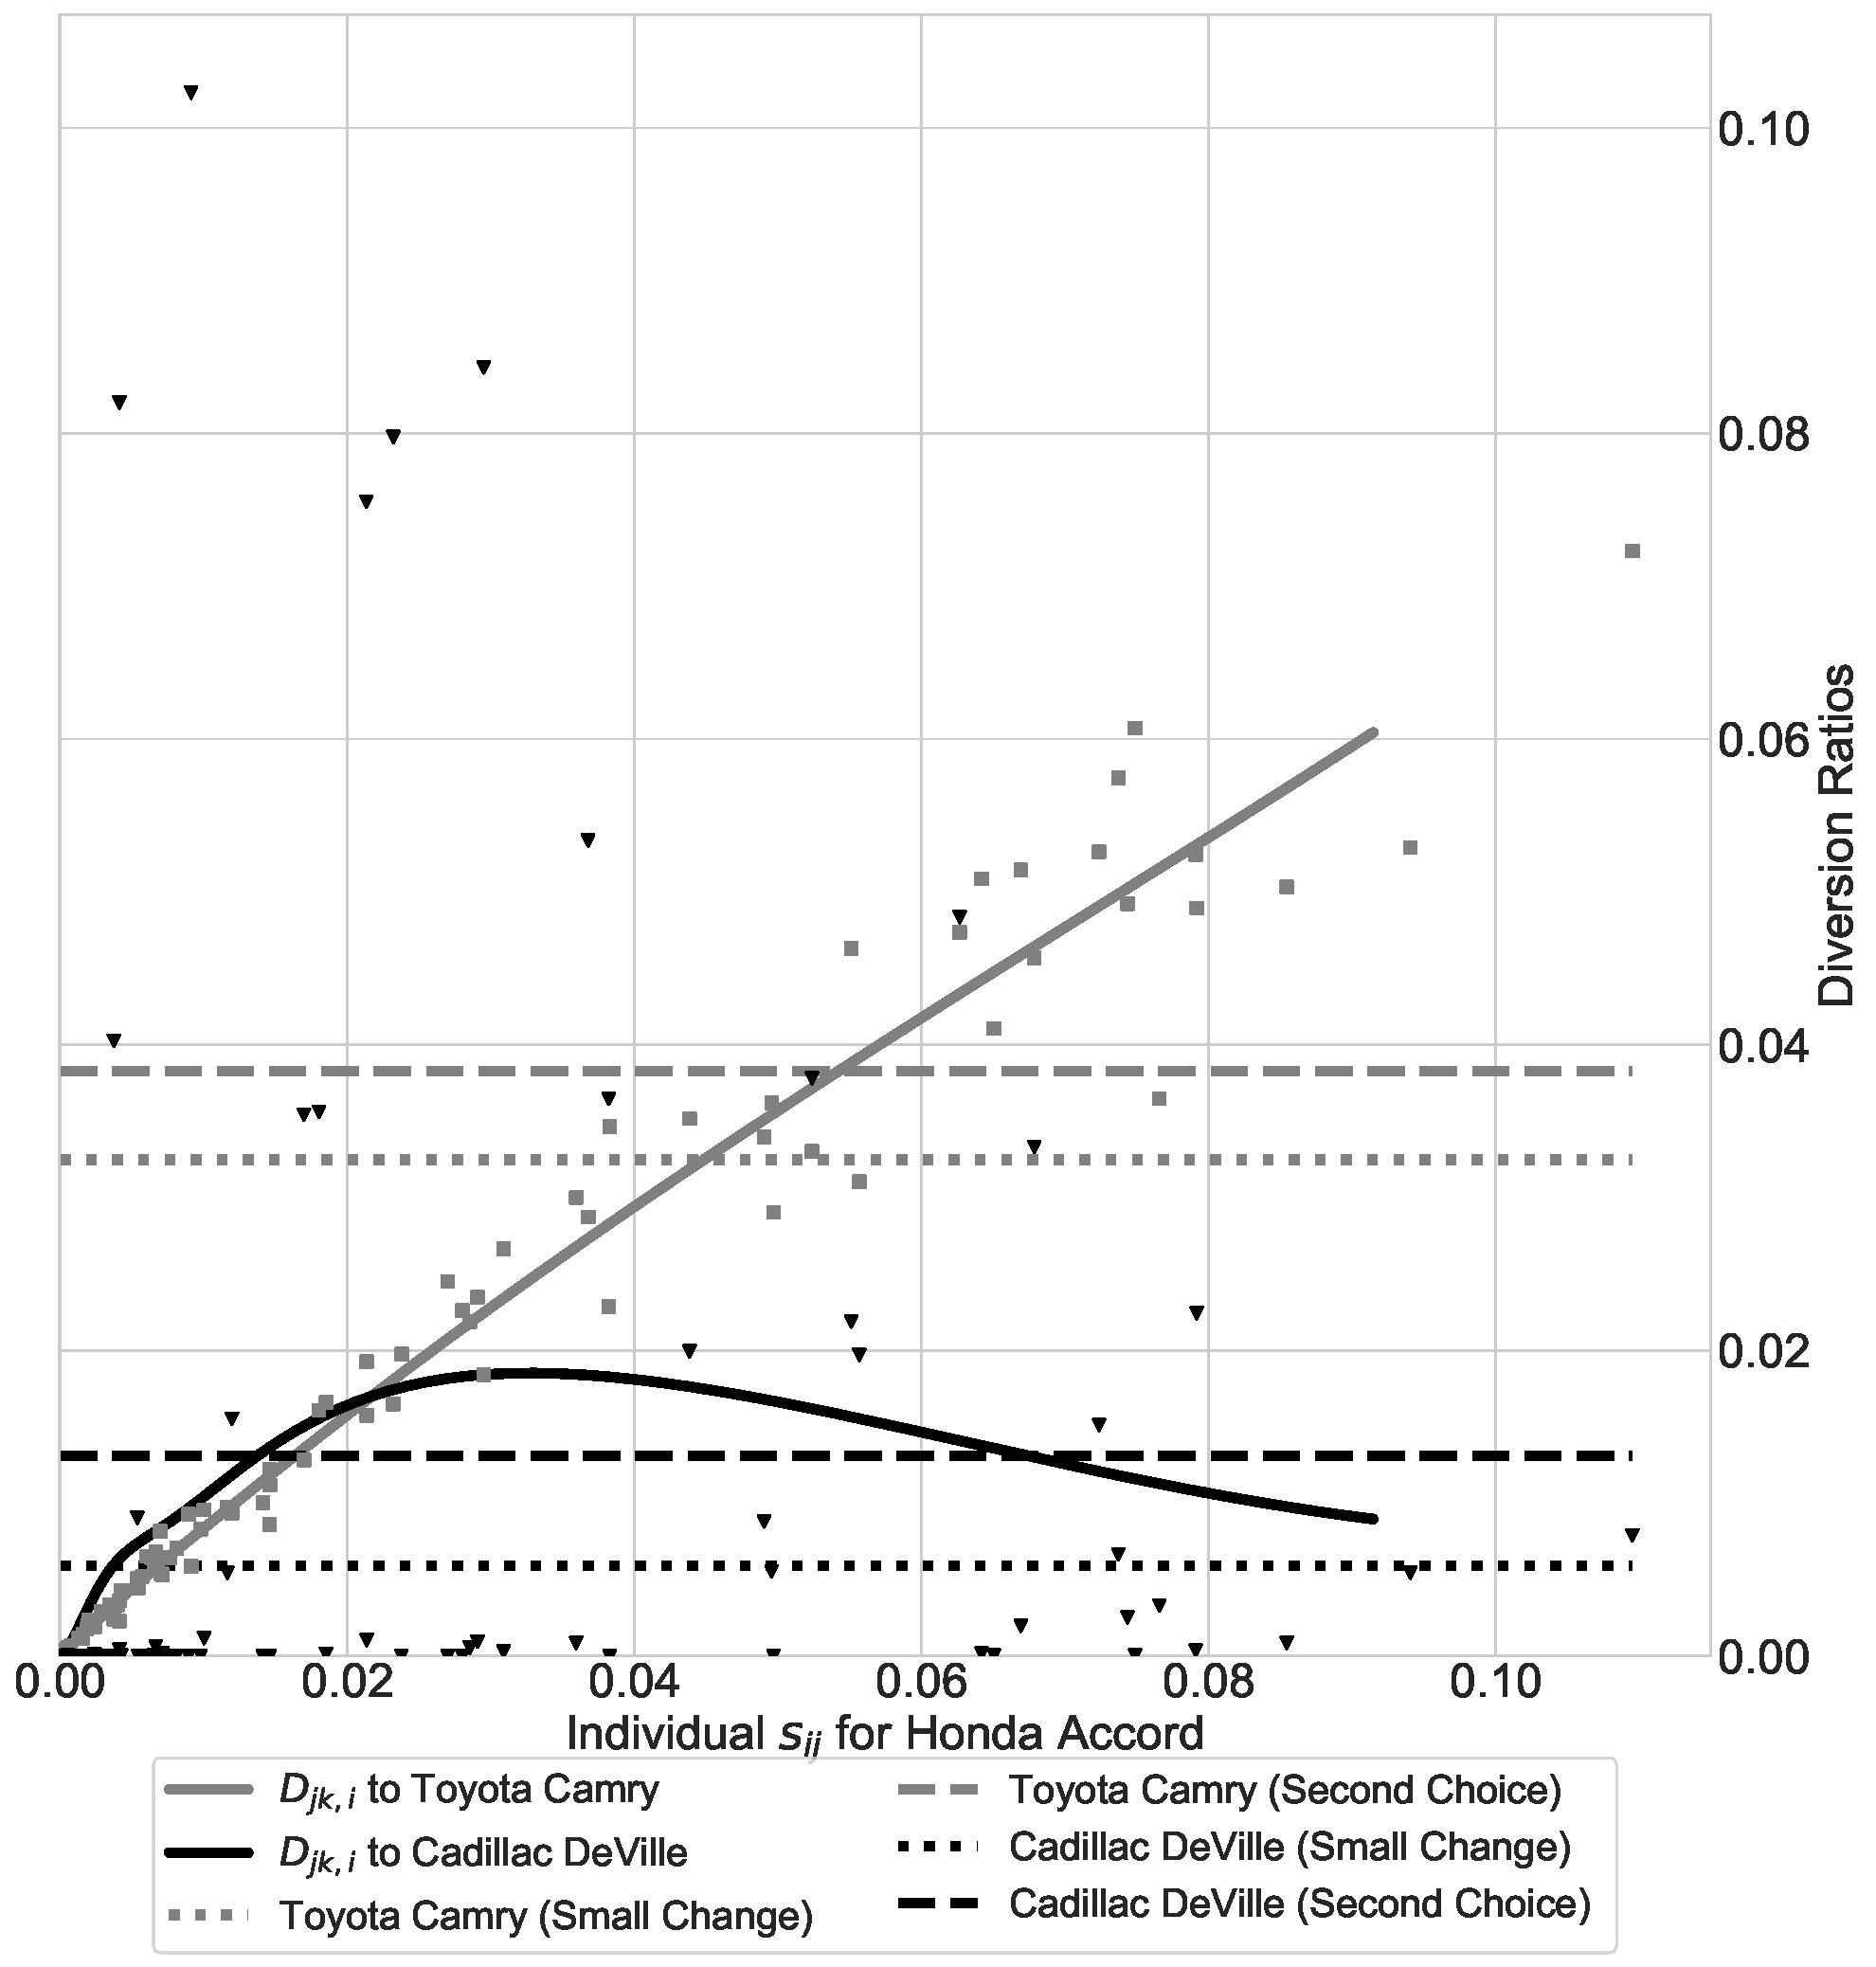
\includegraphics[height=2.7in]{./resources/lines_mte_53_113_19.pdf}
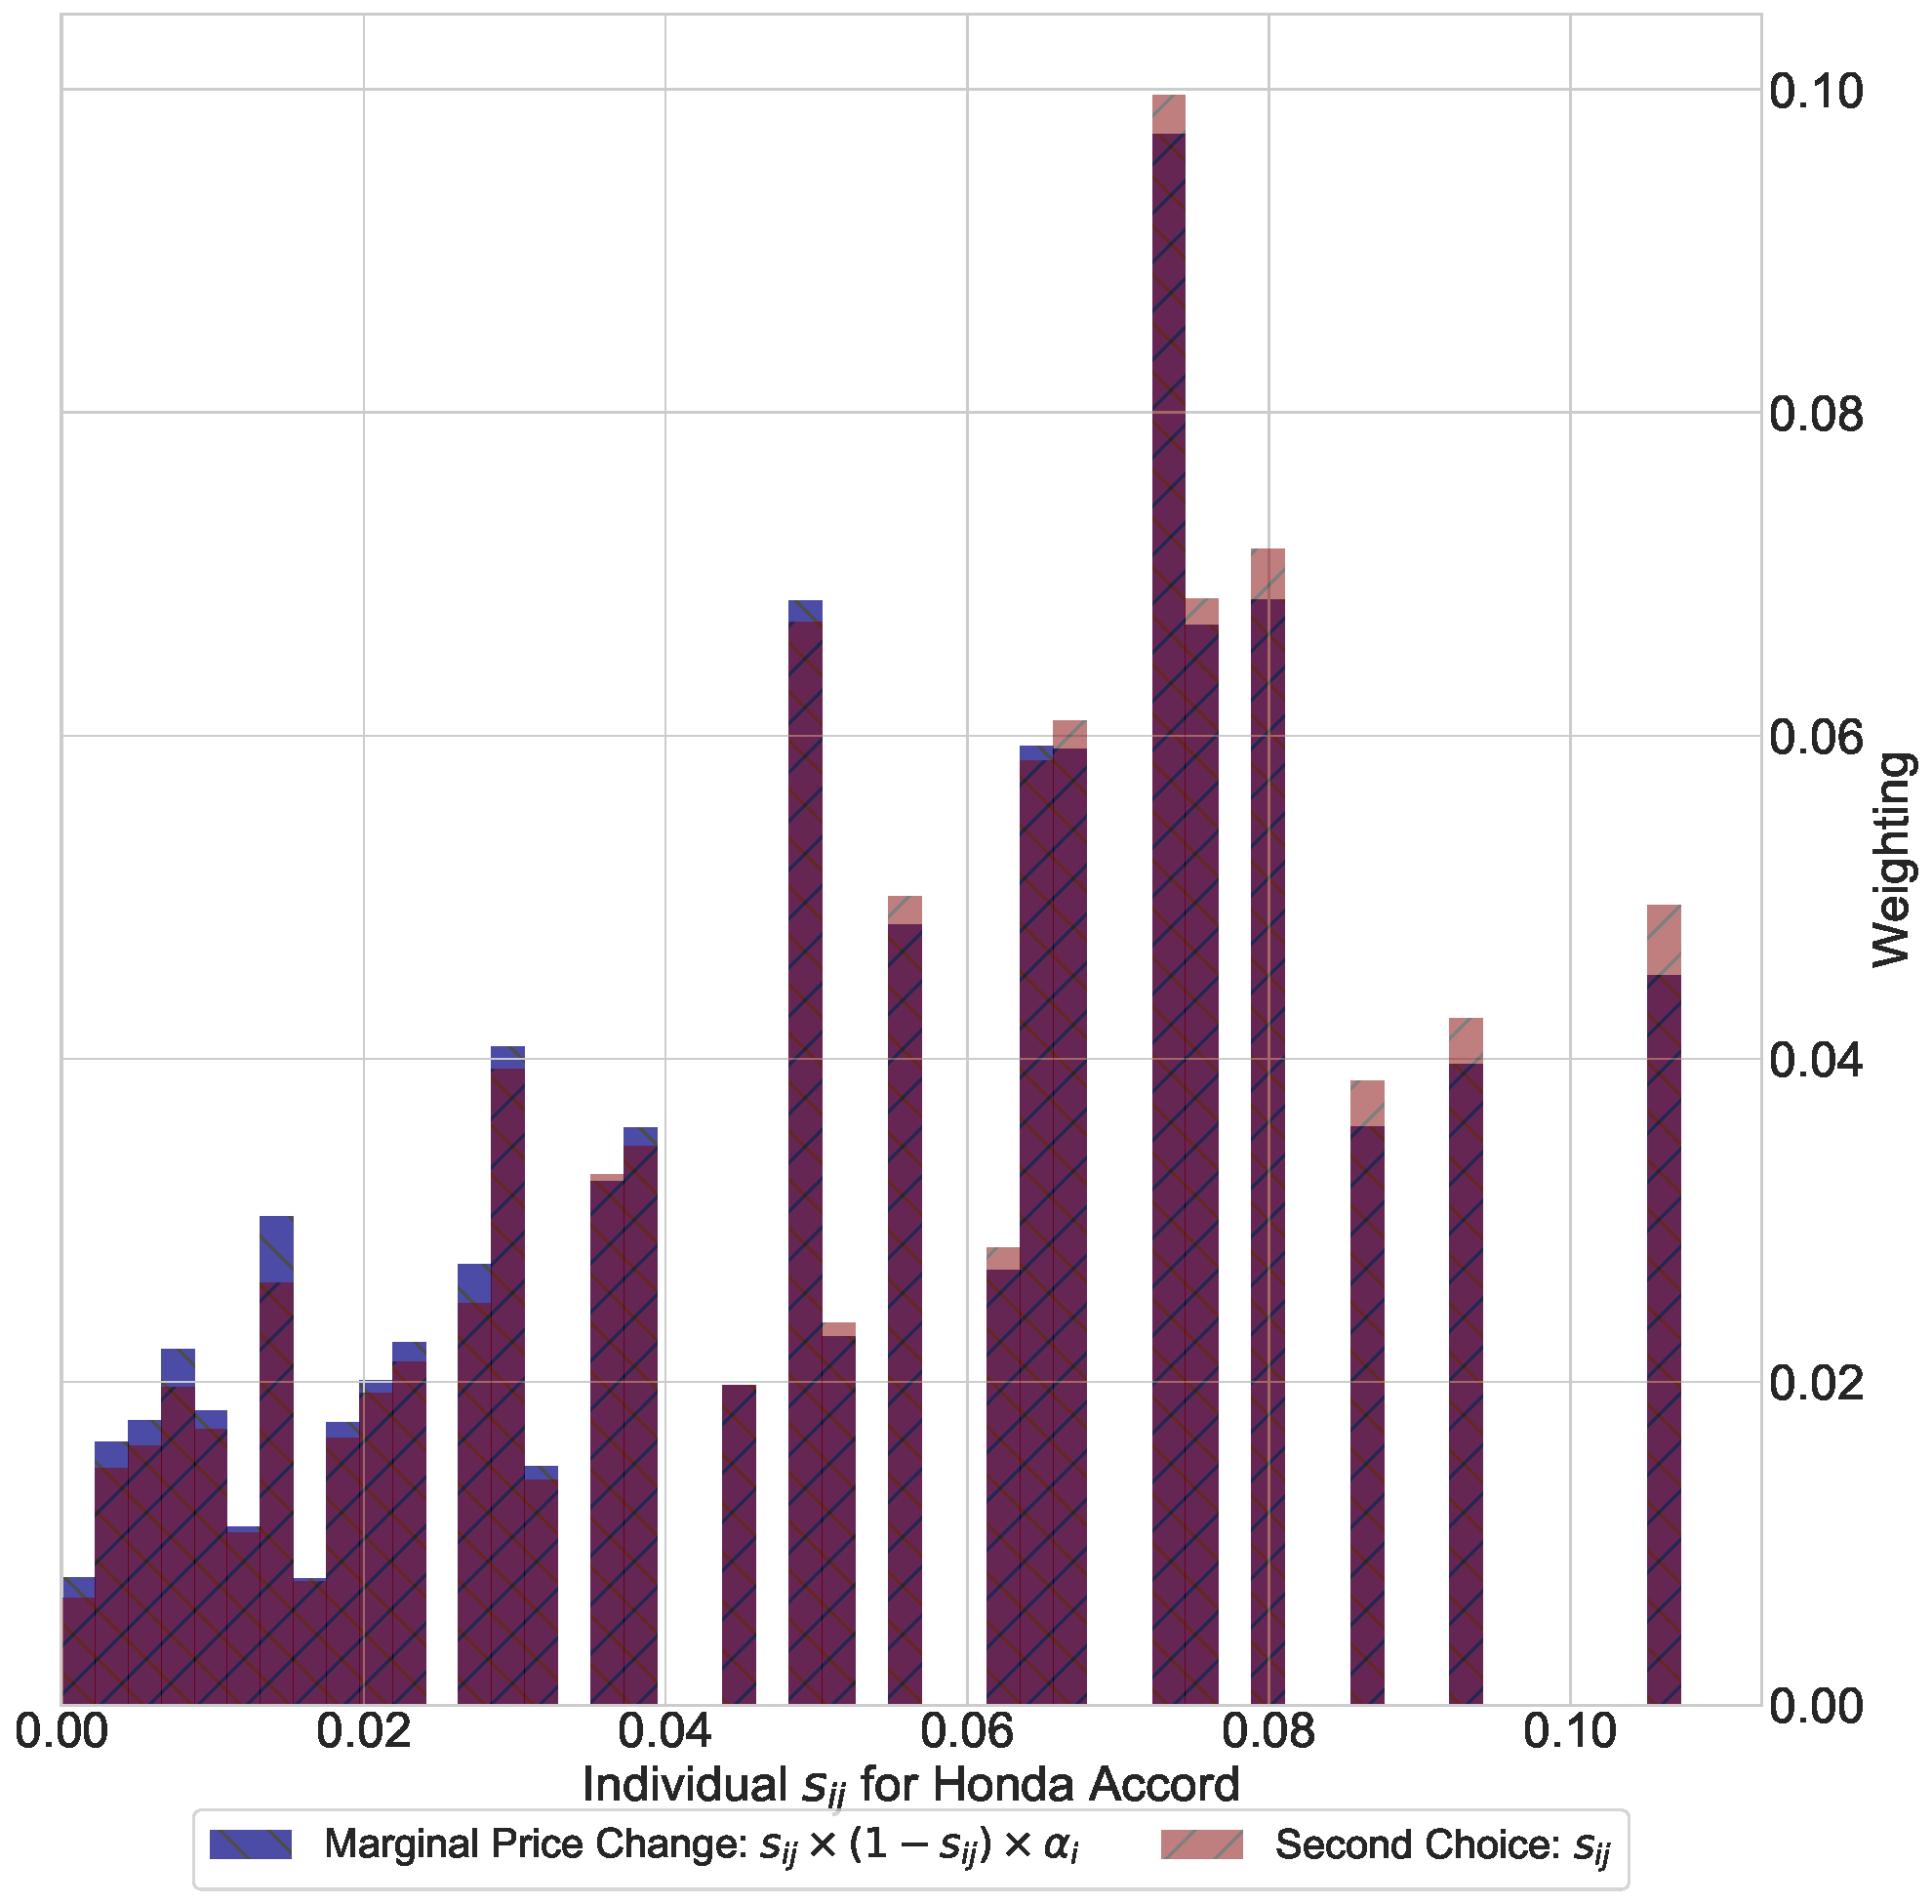
\includegraphics[height=2.7in]{./resources/hist_mte_53_113_19.pdf}
\end{center}
\end{frame}

\end{document}

